\chapter{The CMS Experiment at the Large Hadron Collider}
\section{Introduction}
The Large Hadron Collider (LHC) is a proton-proton ($\Pp\Pp$) accelerator
located at the CERN particle physics laboratory near Geneva, Switzerland. The
LHC is built in the tunnels formerly occupied by the LEP experiment, a
\unit{27}{\kilo\metre} long ring lying on the border between France and Switzerland. Two
beams of protons run in opposite directions around the ring and are made to
collide at four interaction points.

There are four primary experiments at the LHC: \ac{ALICE}, \ac{ATLAS}, \ac{CMS}
and \ac{LHCb}. Each one is constructed around one of the four interaction points
and records the shower of particles produced from the colliding protons. ATLAS
and CMS are large, general purpose detectors designed to search for a variety of
\ac{NP} signatures as well as making higher precision measurements of \ac{SM}
parameters. \ac{ALICE} is designed to examine the products of heavy-ion
collisions (lead-lead) in order to explore the quark gluon plasma and related
physics. Finally, the \ac{LHCb} experiment is optimised for the study of B-meson
decays. These are important for the study of CP violation within the \ac{SM} but
might also provide potential avenues for the discovery of \ac{NP}.

\section{The \acl{LHC}}
The \ac{LHC} is a circular $\Pp\Pp$ synchrotron with a circumference of
\unit{27}{km}. It sits in a tunnel initially constructed for the \ac{LEP}
accelerator buried at a depth of between 50 and \unit{175}{\metre} beneath the
Franco-Swiss border. At full design specifications, 2808 bunches of protons will
circulate around each direction of the ring, colliding at a centre of mass
energy of \unit{14}{\tera\electronvolt}. With a proton bunch spacing of
\unit{25}{\ns}, the \ac{LHC} will eventually achieve a luminosity of
\unit{$10^{34}$}{\rpsquare{\centi\metre}\usk\reciprocal\second}.

\subsection{Accelerator Complex}
The \ac{LHC} ring itself is the final stage in an injector chain utilising a
series of accelerators built at CERN over the last 50 years. Each stage supplies
an incremental increase in the proton (or heavy ion) bunch energy. The first
stage in this chain is a linear accelerator, either the Linac2 for proton
injection or Linac3 during heavy-ion runs. The Linac2 injects protons into the
\ac{PSB} at an energy of \unit{50}{\mega\electronvolt}. Similarly, the ions
proceed first from the Linac3 to the \ac{LEIR} before finally arriving at the
\ac{PS}. From here on, the paths of the protons and heavy-ions are the
same. Proton bunches pass from the \ac{PSB} to the \ac{PS} at an energy of
\unit{1.4}{\giga\electronvolt} and then on to the \ac{SPS} at an energy of
\unit{28}{\giga\electronvolt}. Protons then arrive at the \ac{SPS}, where they
circulate around a ring \unit{2}{\kilo\metre} in diameter, and increasing their
energy to \unit{450}{\giga\electronvolt}. From here, kicker magnets inject the
bunches into the \ac{LHC} itself, where the energy is finally increased to the
design specified \unit{7}{\tera\electronvolt} per beam.
\begin{figure}
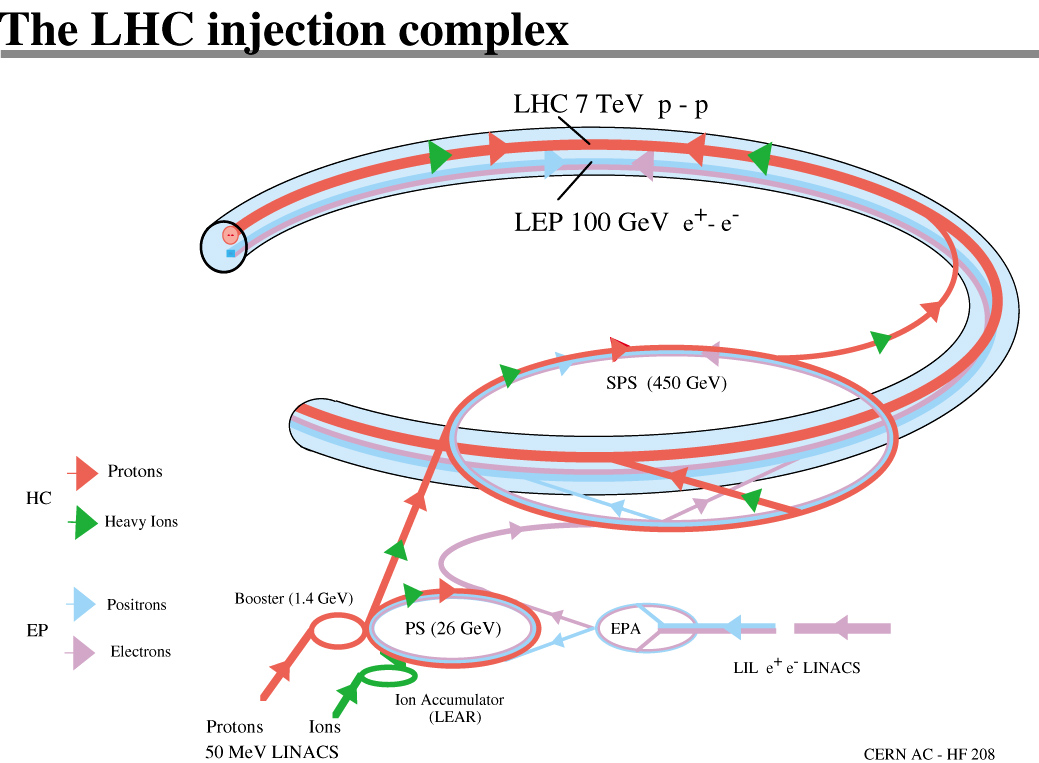
\includegraphics[width=0.9\textwidth]{figures/lhc-pho-1993-008}
\end{figure}

\ctable[
cap=LHC Accelerator Complex,
caption=LHC Accelerator Complex,
mincapwidth=0.5\textwidth,
pos=h
]{lcc}{
\tnote[a]{Heavy-Ions only}
}{\FL
Accelerator & Energy \ML
%
Linac2   & \unit{50}{\mega\electronvolt} \NN
Linac3\tmark[a]   & \unit{4.2}{\mega\electronvolt\per u} \ML
%
\acf{PSB} & \unit{1.4}{\giga\electronvolt} \NN
\acf{LEIR}\tmark[a]   & \unit{??}{\mega\electronvolt\per u} \ML
%
\acf{PS} & \unit{28}{\giga\electronvolt} \NN
\acf{SPS} & \unit{450}{\giga\electronvolt} \NN
\acf{LHC} & \unit{7}{\tera\electronvolt} \LL
}

\section{The \acl{CMS} Experiment}
